\documentclass[10pt]{article}
\usepackage{amsmath,textcomp,amssymb,geometry,graphicx,enumerate,tikz,algorithm,algpseudocode,pifont}
\usetikzlibrary{calc}
\usetikzlibrary{datavisualization}
\usetikzlibrary{datavisualization.formats.functions}


\textheight=9in
\textwidth=7in
\topmargin=-.75in
\oddsidemargin=-0.25in
\evensidemargin=-0.25in

\usepackage{listings}
\lstnewenvironment{codeblock}
    {\lstset{language=Python,
      showspaces=false,
      showtabs=false,
      breaklines=true,
      mathescape=true,
      showstringspaces=false,
      breakatwhitespace=true,
      commentstyle=\textit,
      keywordstyle=\textbf,
      basicstyle=\ttfamily,
      escapechar=`,
      moredelim={**[is][{\color{RoyalBlue}}]{\^^M\\beginsol}{\^^M\\endsol}},
      moredelim={[is][{\color{RoyalBlue}}]{\^^M\\beginexp}{\^^M\\endexp}},
    }}
    {}

\begin{document}
\section*{03/28/2016}

\subsection*{Decision Trees (continued)}

\subsubsection*{Multivariate Splits}
	\begin{itemize}
		\item Split on multiple features at a time.
			\item Find non-axis-aligned splits with other classification algorithms or by generating them randomly.
			\begin{center}
				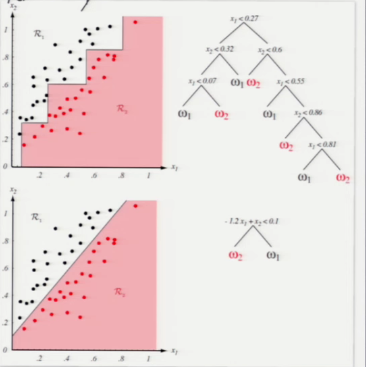
\includegraphics[scale=0.5]{../images/multivariatedecisiontree}
			\end{center}
			\item Need to look at more than one feature.
			\item May gain better classifier at the cost of worse interpretability.
			\item Can limit number of features per split:
				\begin{itemize}
					\item Forward stepwise selection.
					\item Lasso.
				\end{itemize}
	\end{itemize}

\subsubsection*{Decision Tree Regression}
	\begin{itemize}
		\item Creates a piecewise constant regression function.
		\begin{center}
			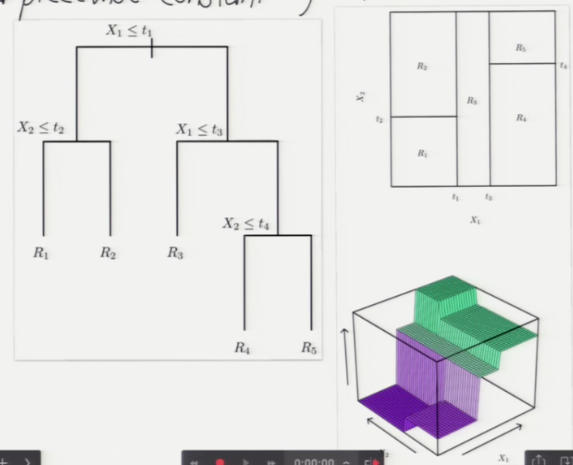
\includegraphics[scale=0.4]{../images/decisionregression}
		\end{center}
		\item $S$ is the set of sample indices that had trickled down to this node of the tree. The more different the $y$ values are the greater the cost should be.
		\item Cost $J(S) = \sum_{i \in S} (y_{i} - \bar{y})^{2}$, where $\bar{y}$ is the mean $y_{i}$ for sample subset $S$.
		\item If all samples in this node agree on the $y$ then the cost is zero.
		\item When we try to split a node, we look at all the different ways we could split a node and we choose whichever minimized the weighted average of the cost functions of the two children.
		\item If you have several points in a leaf average the $y$ values and assign that value.
	\end{itemize}

\subsubsection*{Stopping early}
	\begin{itemize}
		\item Why?
		\begin{itemize}
			\item Limit tree depth (for speed).
			\item Limit tree size (big data sets).
			\item Complete tree may overfit.
			\item Given noise or overlapping distribution, purity of leaves is counterproductive; better to estimate posterior probabilities.
			\begin{center}
				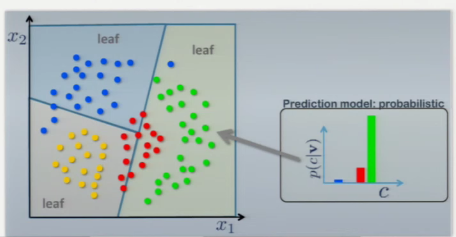
\includegraphics[scale=0.5]{../images/probablitiestree}
			\end{center}
		\end{itemize}
		\item How? Select stopping condition(s):
		\begin{itemize}
			\item Next split doesn't reduce entropy/error enough (dangerous; pruning better).
			\item Most of node's points (e.g. $> 95\%$) have same class.
			\item Node contains few sample points (e.g. $< 10$).
			\item Node covers tiny volume.
			\item Depth too great.
			\item Use (cross)-validation to compare.
		\end{itemize}
		\item Leaves with multiple points return:
		\begin{itemize}
			\item a majority vote or class posterior probabilities (classification)
			\item an average (regression)
		\end{itemize}
	\end{itemize}
	
\subsubsection*{Pruning}
	\begin{itemize}
		\item Grow tree too large; greedily remove each split whose removal improves cross-validation performance. More reliable than stopping early.
	\end{itemize}
	
\subsection*{Ensemble Learning}
\begin{itemize}
	\item Decision trees are fast, simple, interpretable, invariant under scale/translation, robust to irrelevant features.
	\item But not the best at prediction. High variance.
	\item We can take average of output of:
		\begin{itemize}
			\item Different learning algorithms
			\item Same learning algorithm on many training sets.
			\item \underline{Bagging}: same learning algorithm on many random subsamples of one training set.
			\item \underline{Random forests}: Randomized decision trees on random subsamples.
		\end{itemize}
	\item Regression algorithms: take median or mean output.
	\item Classification algorithms: take majority vote or average posterior probabilities.
	\item Use learners with low bias (e.g. deep decision trees).
	\item High variance and some overfitting is okay. Averaging reduces the variance!
	\item Averaging sometimes reduces the bias and increases flexibility; e.g averaging linear classifiers $\rightarrow$ nonlinear decision boundaries.
	\item Hyper-parameters settings usually different than 1 learner.
	\item Number of trees is another hyper-parameter.
\end{itemize}

\subsubsection*{Bagging = Bootstrap Aggregating (Leo Breinman, 1994)}
\begin{itemize}
	\item Given $n$-point training sample, generate random subsample of size $n'$, by sampling with replacement. Same points chosen multiple times; some not chosen.
	\item If $n' = n, \sim 63.2\%$ are chosen.
	\item Build learner. Points chosen $j$ times have greater weight:
		\begin{itemize}
			\item Decision trees: $j$-time point has $j$ x weight in entropy.
			\item SVMs: $j$-time point incurs $j$ x penalty to violate margin.
			\item Regression: $j$-time point incurs $j$ x loss.
		\end{itemize}
	\item Repeat until $T$ learners. Metalearner takes test point, feeds it into all $T$ learners, returns average/majority output.
\end{itemize}

\subsubsection*{Random Forests}
\begin{itemize}
	\item Random sampling isn't random enough!
	\item Idea: at each split, take random sample of $m$ features (out of $d$). Choose best split from $m$ features. Different random samples for each split. $m \sim \sqrt{d}$ good for classification; $m \sim \frac{d}{3}$ for regression.
	\item Smaller $m \rightarrow$ more randomness, less tree correlation, more bias.
	\item Sometimes test error reduction up to 100's or even 1000's of trees. Advantage much more accurate tree but less interpretability.
	\item Variation: Generate $m$ random multivariate splits (oblique lines, quadrics); choose best split.
\end{itemize}

\end{document}
